\begin{tikzpicture}[x=.4\marginparwidth,y=.4\marginparwidth,>=stealth]
\draw [thick,{\colorone}] (0,1) arc[start angle=90,end angle=270,radius=1];
\draw [thick,{\colorone}] (0,-1) parabola (1,1);
\filldraw (0,1) circle[radius=2pt] node [below] {$A$};
\filldraw (1,1) circle[radius=2pt] node [right] {$B$};
\filldraw (0,-1) circle[radius=2pt] node [above] {$D$};
\draw (-1,0) node [right] {$C_1$};
\draw (.5,-.5) node [right] {$C_2$};
\draw [thick,->,{\colorone}] (-1,0)--(-1,-.01);
\draw [thick,->,{\colorone}] (.5,-.5)--(.51,-.48);
\draw (-1,0) node {\phantom{M}};
%\begin{axis}[width=\marginparwidth+25pt,tick label style={font=\scriptsize},axis y line=none,axis x line=none,name=myplot,%
			%%xtick={-2,-1,1,2},
%%			ytick={-1,1,2,3},
%%			minor y tick num=1,
%%			extra x ticks={-6.28,-3.14,3.14,6.28},%
%%			extra x tick labels={$-2\pi$, $-\pi$, $\pi$, $2\pi$},
			%ymin=-2,ymax=2,%
			%xmin=-2,xmax=2,%
%%			grid=major
%]
%
%\addplot [thick,{\colorone},smooth,domain=90:270,samples=30] ({cos(x)},{sin(x)});
%\addplot [thick,{\colorone},domain=0:1,samples=30] {x^2-1};
%%\addplot [thick,{\colorone},domain=5.01:6.5,samples=50] {1/((x-3)*(x-5)^2)};
%
%%\draw [{\colorone},dashed] (axis cs:5,105) -- (axis cs:5,-105);
%
%
%\end{axis}
%%\node [right] at (myplot.right of origin) {\scriptsize $x$};
%%\node [above] at (myplot.above origin) {\scriptsize $y$};
\end{tikzpicture}
